%************************************************
\chapter{Elección del Algoritmo}
\label{ch:algorithm}
%************************************************
\citeauthor{yamada2003} \cite{yamada2003} proponen un método para analizar las
dependencias palabra-a-palabra mediante una estrategia \emph{bottom-up} -- de
abajo a arriba. -- Para ello se hace uso de la técnica de \ac{AA}
\acfi{SVM}. Sus experimentos se basan en árboles de dependencias creados a
partir del corpus \ac{PTB}, logrando una precisión superior al 90\% para
dependencias palabra-a-palabra. Aún siendo esta precisión inferior al
\nameref{sec:stateoftheart}, hay que tener en cuenta que este método no utiliza
información sobre la estructura de las frases.

El tipo de anotaciones usadas en este método pueden verse en la
\autoref{fig:deptree}. Esta forma de ilustrar las dependencias palabra-a-palabra
es más sencilla de entender para los anotadores que tengan un amplio
conocimiento del dominio a trabajar, pero carezcan del conocimiento lingüísitco.

\begin{figure}[h]
\resizebox{1.3\textwidth}{!}{%
\begin{tikzpicture}[every node/.style={align=center}]
  \tikzset{
    edge from parent/.style={
      draw,edge from parent
      path={(\tikzparentnode.south)-- +(0,-8pt)-| (\tikzchildnode)}
    },
    frontier/.style={distance from root=350pt} % Align leaf nodes
  }

   \Tree [.S
             [.NP Rolls-Royce\\NNP Motor\\NNP Cars\\NNPS Inc\\NNP ]
             [.VP said\\VBD
                [.SBAR -NONE-
                   [.S
                      [.NP it\\PRP ]
                      [. VP expects\\VBZ
                         [.S
                            [.NP its\\PRP\$ U.S\\NNP sales\\NNS ]
                            [.VP to\\TO
                               [.VP remain\\VB
                                  [.ADJP steady\\JJ ]
                                  [.PP at\\IN
                                     [.NP
                                        [.QP about\\IN 1200\\CD ]
                                        cars\\NNS
                                     ]
                                  ]
                               ]
                            ]
                         ]
                      ]
                   ]
                ]
             ]
         ]
\end{tikzpicture}
}
\caption{Estructura en árbol de la frase ``Rolls-Royce Motor Cars Inc. said it
  expects its U.S. sales to remain steady at about 1,200 cars.''}
\label{fig:strtree}
\end{figure}

\begin{figure}[h]
   \begin{tikzpicture}[every node/.style={align=center},level distance=2cm]
   \tikzset{edge from parent/.append style={<-, >=latex,thick}}
   \Tree [.said\\VBD 
             [.Inc.\\NNP Rolls-Royce\\NNP Motor\\NNP Cars\\NNPS ]
             [.expects\\VBZ it\\PRP
                [.remain\\VB
                   [.sales\\NNS its\\PRP\$ U.S\\NNP ]
                   to\\TO
                   steady\\JJ 
                   [.at\\IN [.cars\\NNS [.about\\IN 1200\\CD ] ] ]
                ]
             ]
           ]
   \end{tikzpicture}
   \caption{Árbol de parseo de dependencias}
   \label{fig:deptree}
\end{figure}
%*****************************************
%*****************************************
%*****************************************
%*****************************************
%*****************************************
